% !TeX root = ../../main.tex
\chapter{Implementation}
\label{chapter:scafi3-arch-reification}

This chapter discusses the instantiation of the proposed abstract architecture described in \Cref{chapter:contribution} to ScaFi3.
%
\todo{link to de luigi thesis for pure core module, that is not part of this work}

\todo{description of the flow}

\todo{high level architecture modules view}

\todo{project structure - shared, jvm-native, js-native, js, native, jvm and expect/actual Scala mechanism}

\section{High level architecture}

The overview of the ScaFi3 architecture is shown in \Cref{fig:scafi3-architecture}, highlighting the main modules and their relationships.
%
\begin{figure}
    \centering
    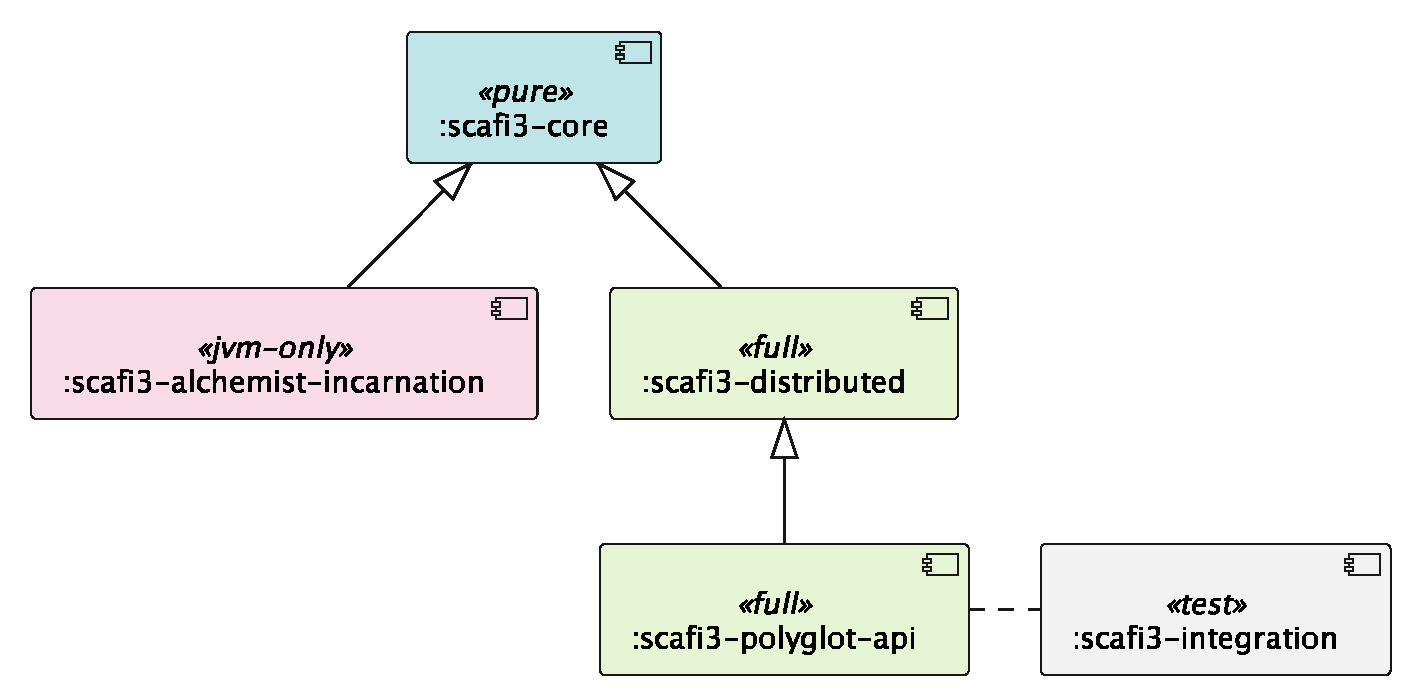
\includegraphics[width=0.7\textwidth]{resources/schemas/scafi3-architecture.eps}
    \caption{UML component diagram of the ScaFi3 architecture.}
    \label{fig:scafi3-architecture}
\end{figure}

\section{Infrastructure module}

\subsection{Distribution module}

Enabling distribution in ScaFi3 requires implementing an abstract network manager that is able to send and receive Value Trees \todo{in context add Value Tree} from and to neighbor devices.
%
The AC framework abstract over the specific protocol used to communicate with neighbors and their discovery mechanism, allowing the implementation of different network managers for different protocols and scenarios.

As an initial step in ScaFi3's evolution toward full-featured distributed capabilities, a socket-based network manager has been implemented. 
%
This foundation layer employs stream, TCP-based connection-oriented sockets, intentionally prioritizing core communication reliability over advanced distributed features, which remain subjects for future work.
%
Indeed, despite the low-level nature of sockets, they provide a foundational abstraction layer that many higher-level protocols ultimately rely upon (such as HTTP, MQTT, etc.), making them a suitable starting point for building extensible communication mechanisms.
%
Consequently, as shown in \Cref{fig:socket-network-manager-architecture}, each device is bound to a specific endpoint (IP address and port) and communicates point-to-point with its neighbors.
%
\begin{figure}
    \centering
    \includegraphics[width=\textwidth]{resources/img/socket-network-manager.pdf}
    \caption{Socket-based network manager high level architecture.}
    \label{fig:socket-network-manager-architecture}
\end{figure}

The UML class diagram of the socket-based network manager is shown in \Cref{fig:socket-network-manager-design}.
%
It adopts an asynchronous design leveraging Scala's Future-based API and comprises two primary active components that operate concurrently to handle bidirectional communication:
%
\begin{itemize}
    \item the incoming connection \texttt{Listener}, continuously listening for incoming messages from neighbor devices. Received messages are stored in a thread-safe \texttt{Map} that retains only the most recent message from each neighbor, according to a configurable \texttt{Retention Policy} that defines, in absence of new messages, how long a message should be retained before being discarded. The up-to-date view of all the received neighbor messages, a.k.a. their Value Trees, is made available to the ScaFi Engine through the \texttt{receive} method at the beginning of each round of computation;
    \item the outgoing message channel, providing a non-blocking interface for message transmission. Upon the end of each round of computation, the ScaFi Engine invokes the \texttt{send} method of the network manager to dispatch the device's current Value Tree to all its neighbors. For each neighbor, the corresponding Value Tree is pushed through the channel and, asynchronously, dispatched to the corresponding destination. To resolve neighbor addresses the socket-based network manager is mixed in with a \texttt{NeighborhoodResolver}, which provides the necessary endpoint resolution capabilities.
\end{itemize}
%
This dual component design ensure that both incoming and outgoing communications proceed without blocking, a pre-condition for targeting JavaScript environments and at the same time maintain system responsiveness.
%
\begin{figure}
    \centering
    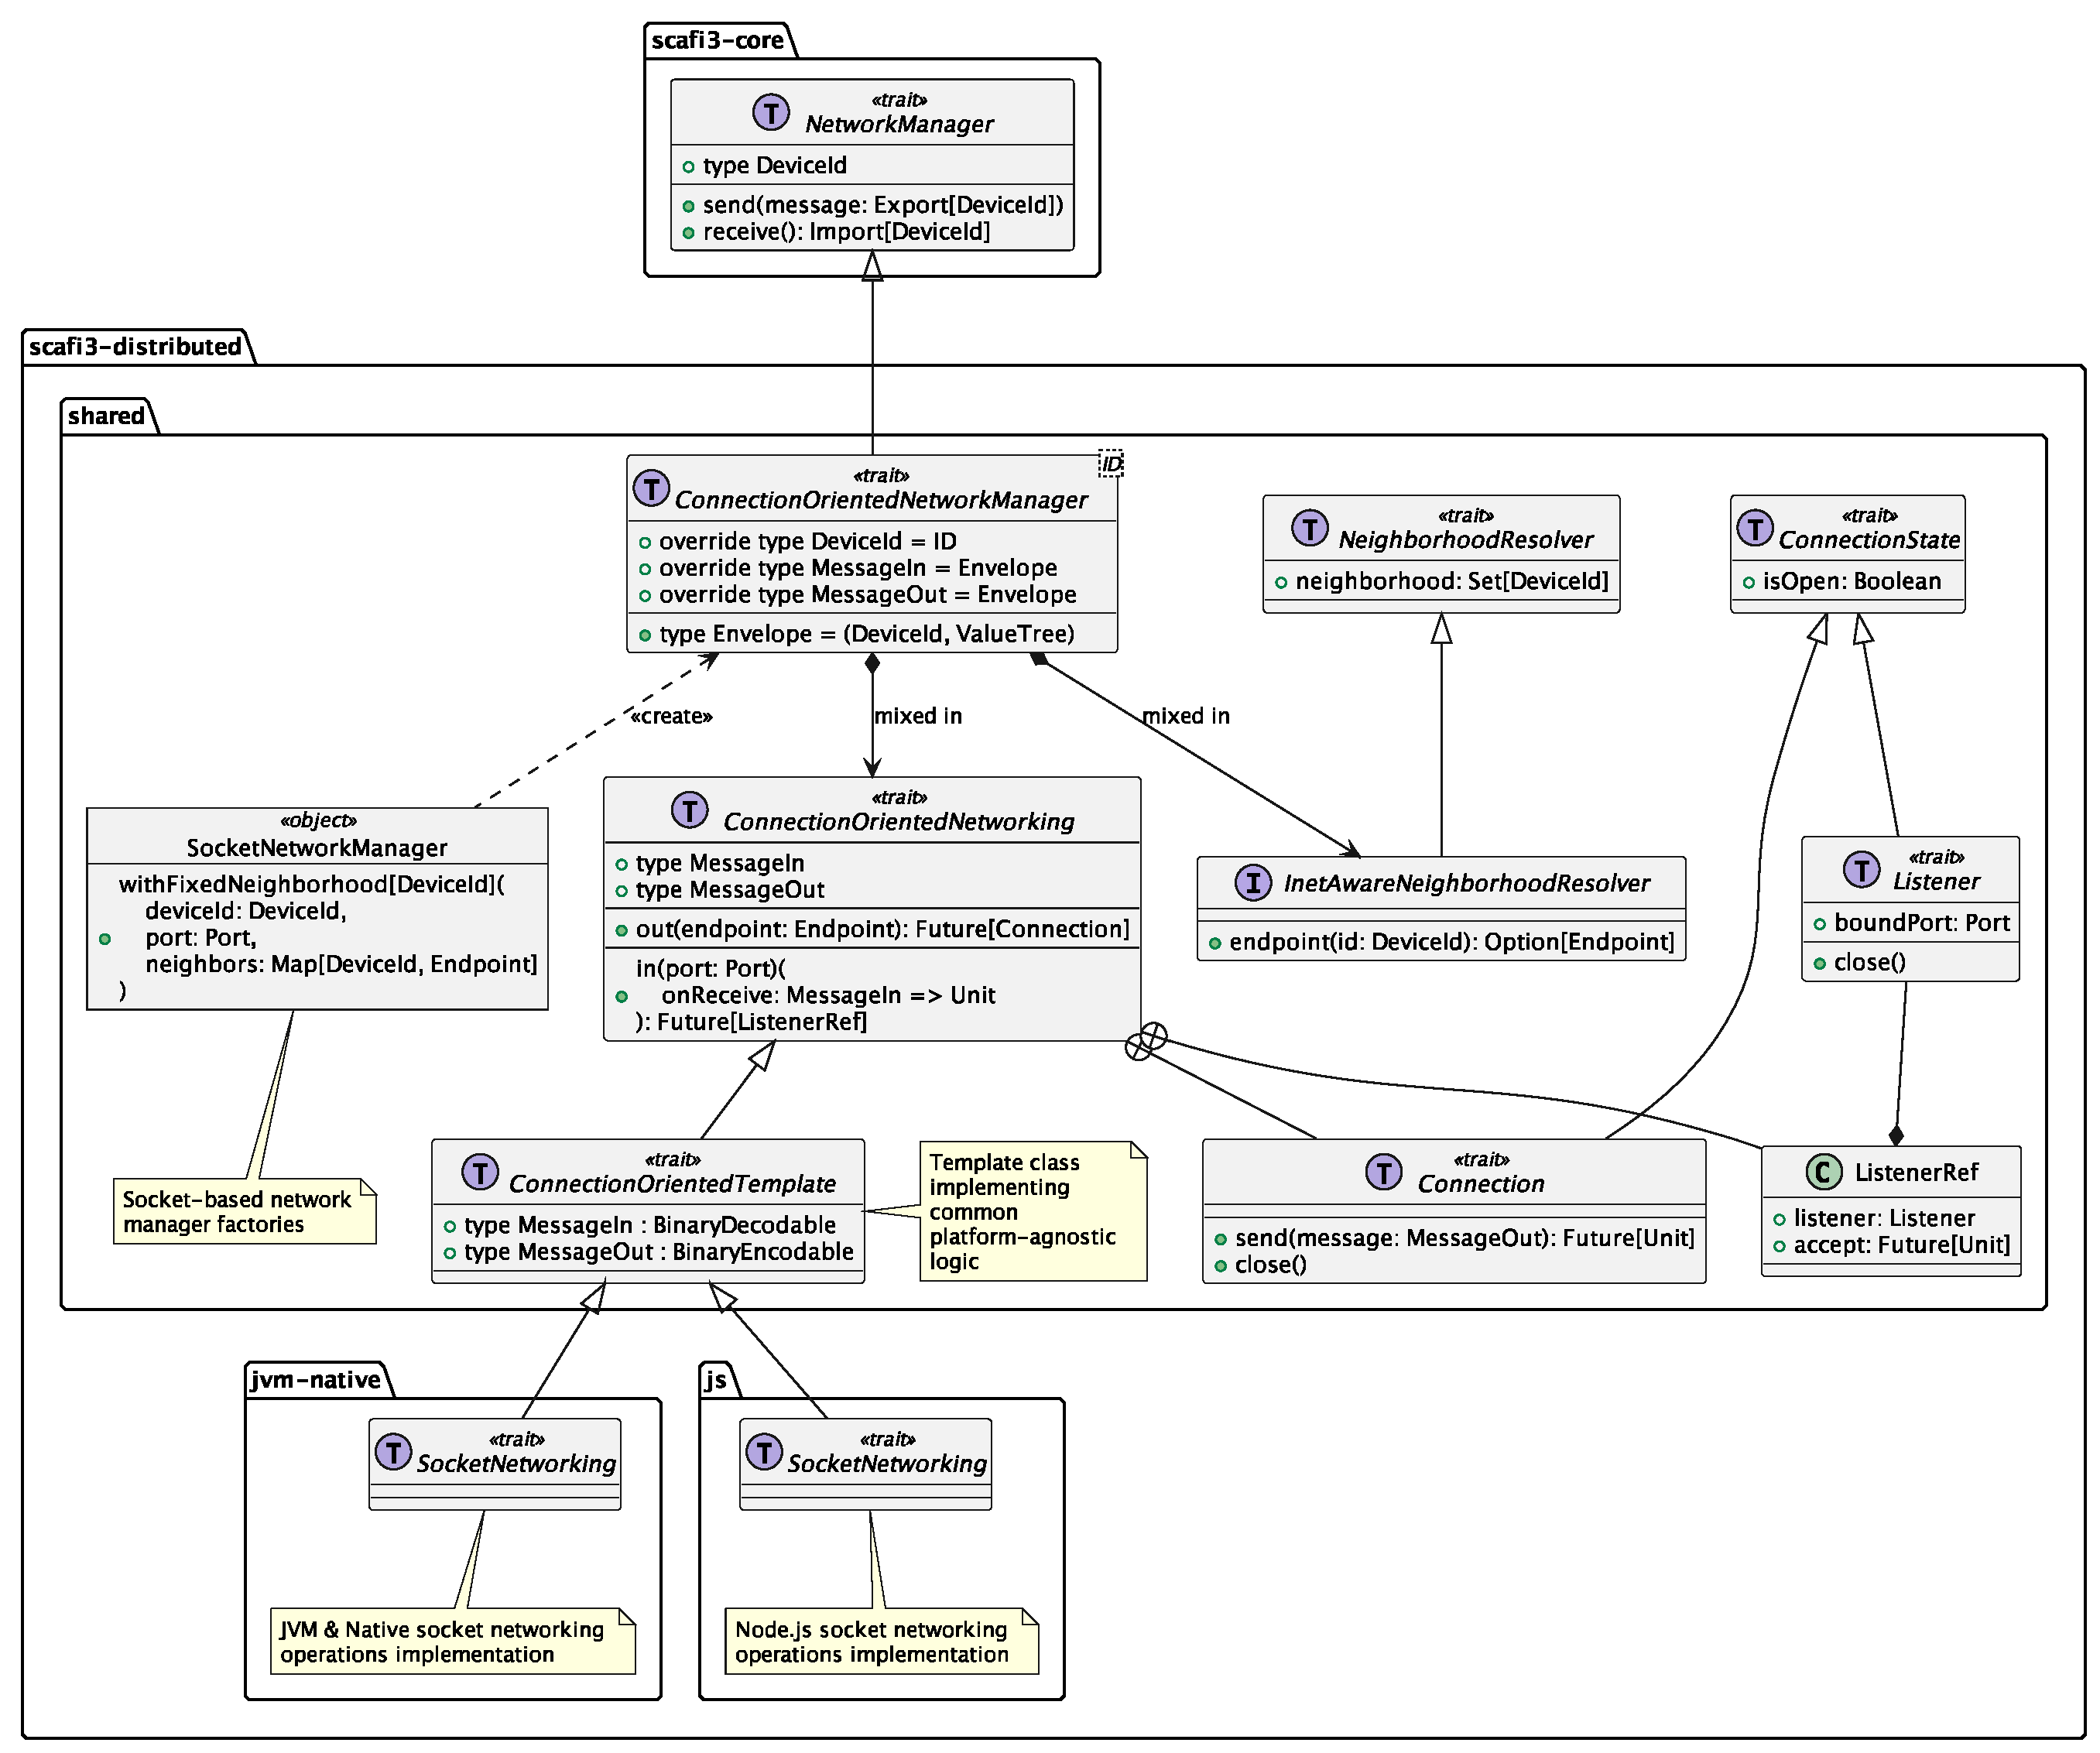
\includegraphics[width=\textwidth]{resources/schemas/socket-distribution.eps}
    \caption{UML diagram of the socket-based network manager design.}
    \label{fig:socket-network-manager-design}
\end{figure}

Remote socket-based communication logic are demanded to the \texttt{ConnectionOrientedNetworking} trait and their platform-specific implementations.
%
Since the absence of a cross-platform socket library supporting both client and server socket programming, two distinct implementations have been provided:
%
\begin{itemize}
    \item one for JVM and Native platforms, leveraging the \texttt{java.net} package available in the standard library. This has been made possible by Scala Native, which have reimplemented the \texttt{java.net} package to provide socket programming capabilities on native platforms. Programmers can thus use the same API on both JVM and Native platforms without any code divergence like they would do in pure Scala JVM applications;
    \item one for JavaScript platforms, leveraging the \texttt{Node.js} library API. For this, the \texttt{net} module of Node.js has been used, through a Scala.js facade that enables calling the Node.js API from Scala.js code. A portion of this facade is shown in \Cref{lst:js-sockets-facade}. This is essentialy the transposition of Node.js API definitions into Scala trait and classes using Scala.js types, annotations and placeholders that, when linked, allow Scala.js code to call the underlying Node.js API.
\end{itemize}

\lstinputlisting[
    language=Scala, 
    label={lst:js-sockets-facade},
    caption={Portion of the Scala.js facade for the Node.js \texttt{net} module.},
    linerange={46-54},
]{resources/code/JSSocketsFacade.scala}

Despite targeting all three platforms, the design differs only in platform-specific networking logic, isolated within respective \texttt{SocketNetworking} traits. 
%
This separation leverages Scala's mixin composition and the template method pattern, defining common logic in abstract trait (\texttt{ConnectionOrientedTemplate}) while deferring platform-specific details to specialized implementations.

\subsection{Serialization binding}

The second crucial responsibility of the infrastructure module is to provide serialization and deserialization capabilities to exchange messages between devices.

As already discusses, in ScaFi3 devices exchange pairs of the Device Identifier and its corresponding Value Tree.
%
Therefore, the infrastructure module must provide mechanisms to serialize and deserialize both the Device Identifier and the Value Tree structures.
%
The main challenge in this regard is that Value Trees are structures that can contain arbitrary user-defined data types as values that need to be serialized but whose type cannot be known in advance.
%
Therefore, it is not possible to provide a ready-to-use fit-for-all serialization mechanism for Value Trees since the serialization of user-defined data types depends on the specific data type used by the library users.

To overcome this challenge, the following protocol is adopted (exemplified in \Cref{fig:serde-value-trees}):
%
\begin{enumerate}
    \item during the execution of the aggregate program, when the Value Tree is built, each value is inserted as encoded using a specific serialization format (e.g., JSON, Byte Array, etc.) provided by the library user. This is possible since, during the evaluation of the Aggregate constructs, the type information of the exchanged values is known at compile time;
    \item at the end of each round of computation, when the Value Tree is ready to be sent to neighbors, the Value Tree is serialized as a whole structure, leveraging the fact that all values are already encoded in a specific-serialization format;
    \item upon receiving a Value Tree from a neighbor device, the Value Tree is deserialized as a whole structure, obtaining a Value Tree where the values are still encoded in the specific serialization format;
    \item finally, assuming the neighbor device is aligned, when evaluating the same Aggregate construct that produced the value, the value is decoded from the specific serialization format back to the original data type, leveraging the type information known at compile time.
\end{enumerate}
%
\begin{figure}
    \centering
    \includegraphics[width=\textwidth]{resources/img/serde-value-trees.pdf}
    \caption{Exemplification of the serialization/deserialization protocol for Value Trees.}
    \label{fig:serde-value-trees}
\end{figure}

This process requires the library user to provide encoding and decoding functions for each data type that is intended to be exchanged between devices.
%
Moreover, all the API needs to be type safe, ensuring that the encoding and decoding functions are present and correctly matched with the data types being exchanged.

Technically, this is achieved via a combination of Scala 3 \textit{type classes} and \textit{type lambdas} that allow to cleanly express values encoding and decoding requirements as type bounds in the signature of the Aggregate constructs.
%
The core type classes used to express encoding and decoding capabilities are \texttt{Encodable} and \texttt{Decodable}, shown in \Cref{lst:encodable-decodable}.
%
They abstract over both the source and target types of the encoding and decoding operations, allowing to express encoding and decoding capabilities for arbitrary types and serialization formats.
%
These have been further expresses as type lambdas to express encoding and decoding capabilities as type bounds on values of functions dealing with distribution, like presented in \Cref{lst:xc-at-work} for the \texttt{exchange} construct.
%
This ensures, thanks to the \textit{ad-hoc polymorphism}, all distribution-related primitives can only be used with values which have the required encoding and decoding capabilities in scope.

\begin{minipage}{\textwidth}
\lstinputlisting[
    language=Scala, 
    label={lst:encodable-decodable},
    caption={Encodable and Decodable type classes.},
    linerange={3-21},
]{resources/code/Codable.scala}
\end{minipage}

\begin{minipage}{\textwidth}
\lstinputlisting[
    language=Scala, 
    label={lst:xc-at-work},
    caption={Example of encoding and decoding capabilities at work in the \texttt{exchange} construct.},
]{resources/code/ExchangeAggregateContext.scala}
\end{minipage}

User-side, to provide encoding and decoding capabilities for a specific data type and serialization format, it is sufficient to provide implicit instances of the \texttt{Encodable} and \texttt{Decodable} type classes in scope.
%
The Scala compiler will automatically summon the correct instance based on the type information available at compile time, ensuring users to call the distribution-related primitives without having to manually pass encoding and decoding functions around or explicitly specify format types.
%
Examples of user-defined instances of the \texttt{Encodable} and \texttt{Decodable} type classes for different serialization formats are shown in \Cref{lst:user-encodable-decodable}.

\begin{minipage}{\textwidth}
\lstinputlisting[
    language=Scala,
    label={lst:user-encodable-decodable},
    caption={User-defined Encodable and Decodable instances for a custom data type.},
    linerange={39-60},
]{resources/code/Codable.scala}
\end{minipage}

The general implementation of the type classes with respect to the serialization format allows to:
%
\begin{itemize}
    \item leave the choice of the serialization format to the library user, who can choose the most appropriate format for their specific use case. For example, in \Cref{lst:user-encodable-decodable} a production-ready Protobuf-based binary format is provided using ScalaPB\footnote{\url{https://scalapb.github.io}}, a popular Scala library for working with Protocol Buffers;
    \item in non-distributed scenarios, like simulation or local testing, or where the distributed primitives are used only to make the state evolve over rounds without actual neighbor communication, like in the \texttt{evolve}, use in-memory Codable instances that do not perform any transformation on the messages, leaving them as-is. Moreover, leveraging Scala 3 inline givens, the compile is able to completely eliminate encoding and decoding operations at compile time in such scenarios avoiding any runtime overhead.
\end{itemize}

\begin{figure}
    \centering
    \includegraphics[width=0.7\textwidth]{resources/img/protobuf-programming-workflow.pdf}
    \caption{}
    \label{fig:protobuf-programming-workflow}
\end{figure}


% \subsection{Platform-specific library abstraction layers}

% \section{Implementation challenges and solutions}
